% !TEX encoding = UTF-8 Unicode

\documentclass[12pt,a4j,titlepage]{ltjsarticle}
\usepackage{semi}
\usepackage{here}
\usepackage{listings}

% \title{}
% \author{}
% \date{}

\begin{document}

\begin{titlepage}
  \begin{center}
  
    \vspace*{20truept}
    
    {\LARGE 2022年度 卒業論文} 
    
    \vspace*{75truept}
    
    {\Huge  VRデートアプリの提案} %論文タイトル

    \vspace{10truept}

    {\Huge } %論文タイトル 長い場合 改行1

    \vspace{10truept}

    {\Huge } %論文タイトル 改行2

    \vspace{85truept}
    
    {\LARGE 指導教員 須田 宇宙 准教授}
    
    \vspace{60truept}
    
    {\LARGE 千葉工業大学 情報ネットワーク学科}
    
    \vspace{15truept}
    
    {\LARGE 須田研究室}
    
    \vspace{70truept}
    
    {\LARGE 1932158 氏名 小池 周平 } % 氏名は消さない 学生番号 氏名 名前

    \vspace{70truept}
    
  \end{center}
  \begin{flushright}

    {\LARGE 提出日 2023年1月17日}
  
  \end{flushright}
\end{titlepage}

\setcounter{tocdepth}{3}
% 目次の出力
\tableofcontents
% 表目次
\listoftables
% 図目次
\listoffigures
\clearpage

\section{緒言}\label{緒言}
%背景
2015年9月に開催された「国連持続可能な開発サミット」でSDGsが掲げられた.この中に少子化も含まれており,その要因は,晩婚化の進展\cite{sasaki2012},交際率・婚姻率の減少\cite{naikakufu2019}などとされている.
実際に日本では,20年間で平均初婚年齢は2.6歳(男性)/3.1歳(女性)増加している.
しかし,結婚意欲は僅かに減少している程度でほぼ変化していない.
すなわち,「結婚はしたいけれど,良い相手に恵まれない」との考えが大多数を占めている\cite{naikakufu2019}.
これは「出会いの場の減少」と「交際への不安」と言い換える事ができる.
過去には学校や職場,友人を通じた出会いが有ったが,最近では出会いの場としてSNSを活用する者やマッチングアプリの利用者が増加している.
近年のマッチングアプリの利用者は増加傾向にあり,2022年での婚姻した夫婦の出会いのきっかけは約20\%がマッチングアプリと答え,最も多い割合となった.

%問題点
一方,マッチングアプリは良い印象ではないと感じる人も多く,そもそも知らない人と2人きりで会うことに恐怖を感じたり,初デートに不安を感じるデート未経験者も少なくない\cite{prtimes,yoshimura2020}.

%目的

そこでVR空間を利用して1度仮想的なデートを実施し,直接会うまでをサポートできればデートに対する印象が変わるのではないかと考えた.
本研究では,2人きりで会う恐怖を緩和し,デートに対する不安を軽減するために,仮想空間内でデートする環境を構築することを目的とする.
%また,2022年の内閣府の調査によると20代の男性の4割がデートの経験がないと記載している.\cite{naikakufu2022}
%これは,「出会いの場の減少」と「交際への不安」と言い換えることができる.
%この問題に対して,出会ってからデートに進展するまでをサポートできれば,婚姻率上昇に繋げられるのではないかと考えた.
%よって,出会ってからデートに進展するまでをサポートできれば,婚姻率上昇に繋げられるのではないかと考えた.
\clearpage

\section{少子化について}\label{少子化について}
\subsection{概要}
少子化は先進国の間で大きな問題として扱われている.
日本も例に漏れず,過去の年間出生者数は第2次世界大戦のベビーブーム期の1949年に270万人と第1のピークを記録し,その「団塊」の世代が出産期を迎えて第2のピークとなっていた.
しかしその後は2010年まで一貫して減少している.
さらに今後50年間で4000万人以上も減少すると見込まれていることから早急な解決を必要としている.
\subsection{少子化が引き起こす問題}
世界的には人口増加を辿っており,日本でも大都市における人口過密は著しい.よって減少することは望ましいのではという考えもある.
しかし,子供の減少は将来的な労働者の減少でもあり,経済活動の基礎となる労働供給の減少は長期的な所得の向上を抑制している.
\subsection{少子化の実態}
少子化は晩婚化の進展と交際率・婚姻率の減少が大きな要因とされる.
晩婚化の進展,交際率・婚姻率の減少の推移をそれぞれ表\ref{table:shokon},図\ref{fig:konninn}に示す.
表\ref{table:shokon}からわかるように20年間で男女ともに平均初婚年齢が2.5歳以上増加している.
また,図\ref{fig:konninn}で1970年から2021年の間で婚姻数が半減していることがわかる.
しかし,結婚意欲は図\ref{fig:iyoku}のように18~34歳の結婚意欲は23年間で男女それぞれ5.5\%と3.5\%程度しか減少していない.
以上の推移から\ref{緒言}で示したように「結婚はしたいけれど,良い相手に恵まれない」との考えが大多数を占めている\cite{naikakufu2019}.
\begin{table}[h]
\centering
  \caption{平均初婚年齢}
  \label{table:shokon}
  \begin{tabular}{rrr}
   & 夫(歳) & 妻(歳) \\
  平成7年 & 28.5 & 26.3 \\
  平成17年 & 29.8 & 28.0 \\
  平成23年 & 30.7 & 29.0 \\
  平成24年 & 30.8 & 29.2 \\
  平成25年 & 30.9 & 29.3 \\
  平成26年 & 31.1 & 29.4 \\
  平成27年 & 31.1 & 29.4 \\
  \end{tabular}
  \end{table}
%clip,width=85mm,height=55mm
\begin{figure}[h]
\begin{center}
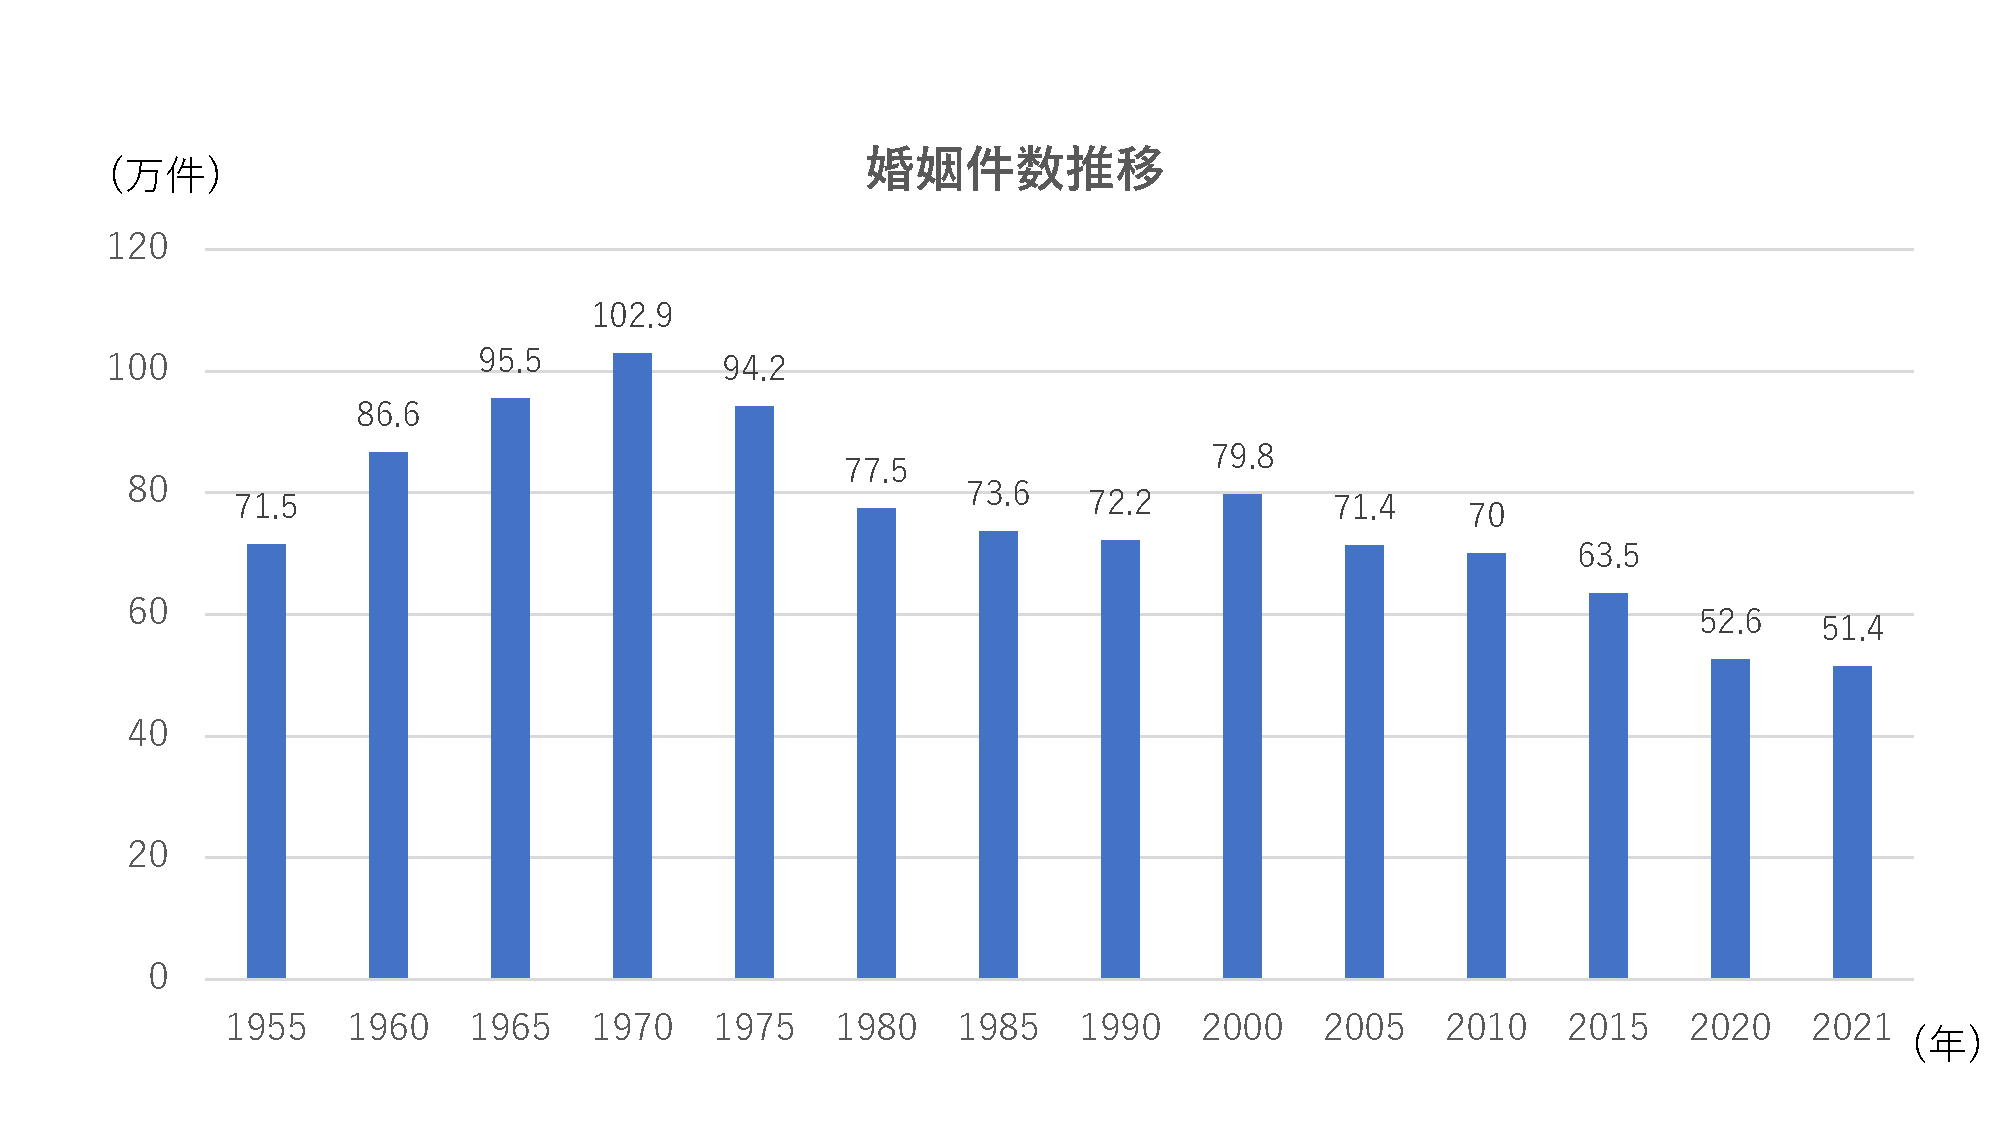
\includegraphics[keepaspectratio, scale=0.5]{koninnsuii.pdf}
\end{center}
 \caption{婚姻数の推移}
 \label{fig:konninn}
\end{figure}

\begin{figure}[h]
\begin{center}
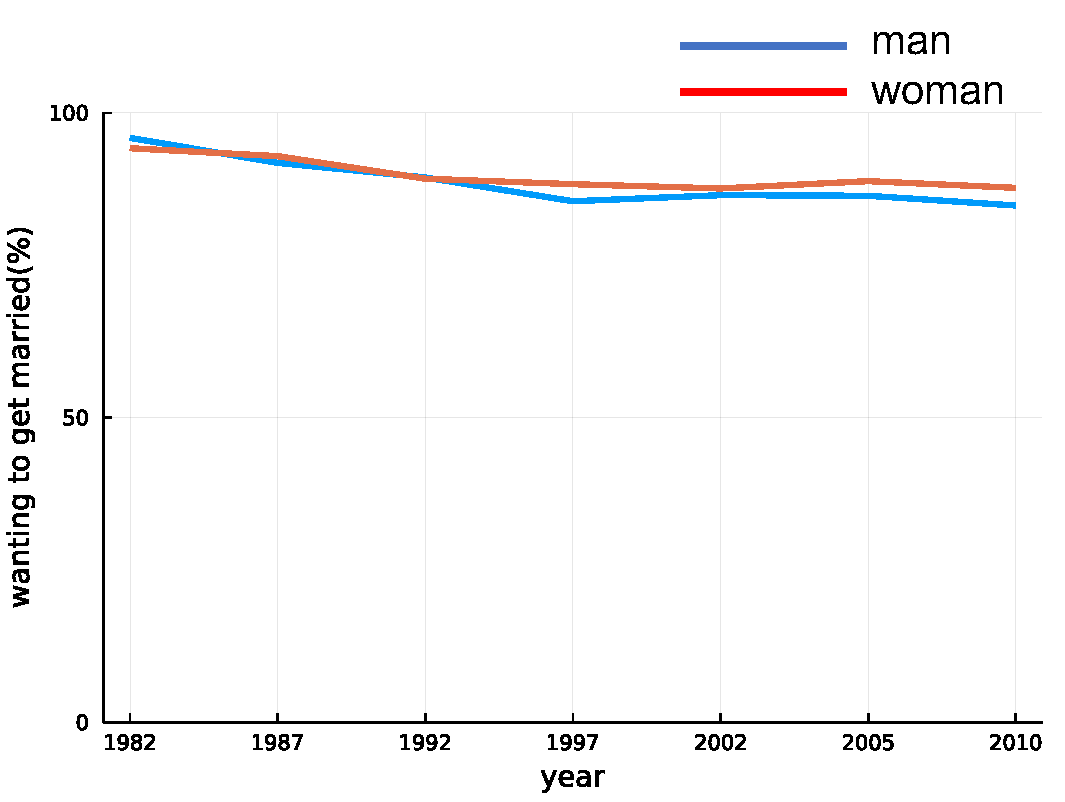
\includegraphics[keepaspectratio, scale=0.7]{preview.pdf}
\end{center}
 \caption{結婚意欲の推移}
 \label{fig:iyoku}
\end{figure}

\clearpage

\section{マッチングアプリについて}
\subsection{概要}
マッチングアプリとは異性・同性の隔てなくインターネット回線を通じてアプリに参加している不特定多数のユーザー間で出会いを作るための仕組みのことである.
\subsection{懸念点}
出会いの場の減少から,多くの社会人がマッチングアプリを利用している.
図\ref{fig:mattingu}は2022年に実施した1620人を対象とした夫婦の出会いのきっかけ調査である.約20\%がマッチングアプリで出会ったとされ,きっかけとしては最多のものとなっている\cite{huuhuutyousa}.
一方,マッチングアプリ自体に懸念を抱いている方は多く,マッチングアプリに関する印象アンケートでは「詐欺や宗教勧誘にあいそう」,「犯罪にあいそう」などの回答が多数派であった\cite{prtimes}.
以上のことから,マッチングアプリには怖い等のイメージを抱かれている.

\begin{figure}[h]
\begin{center}
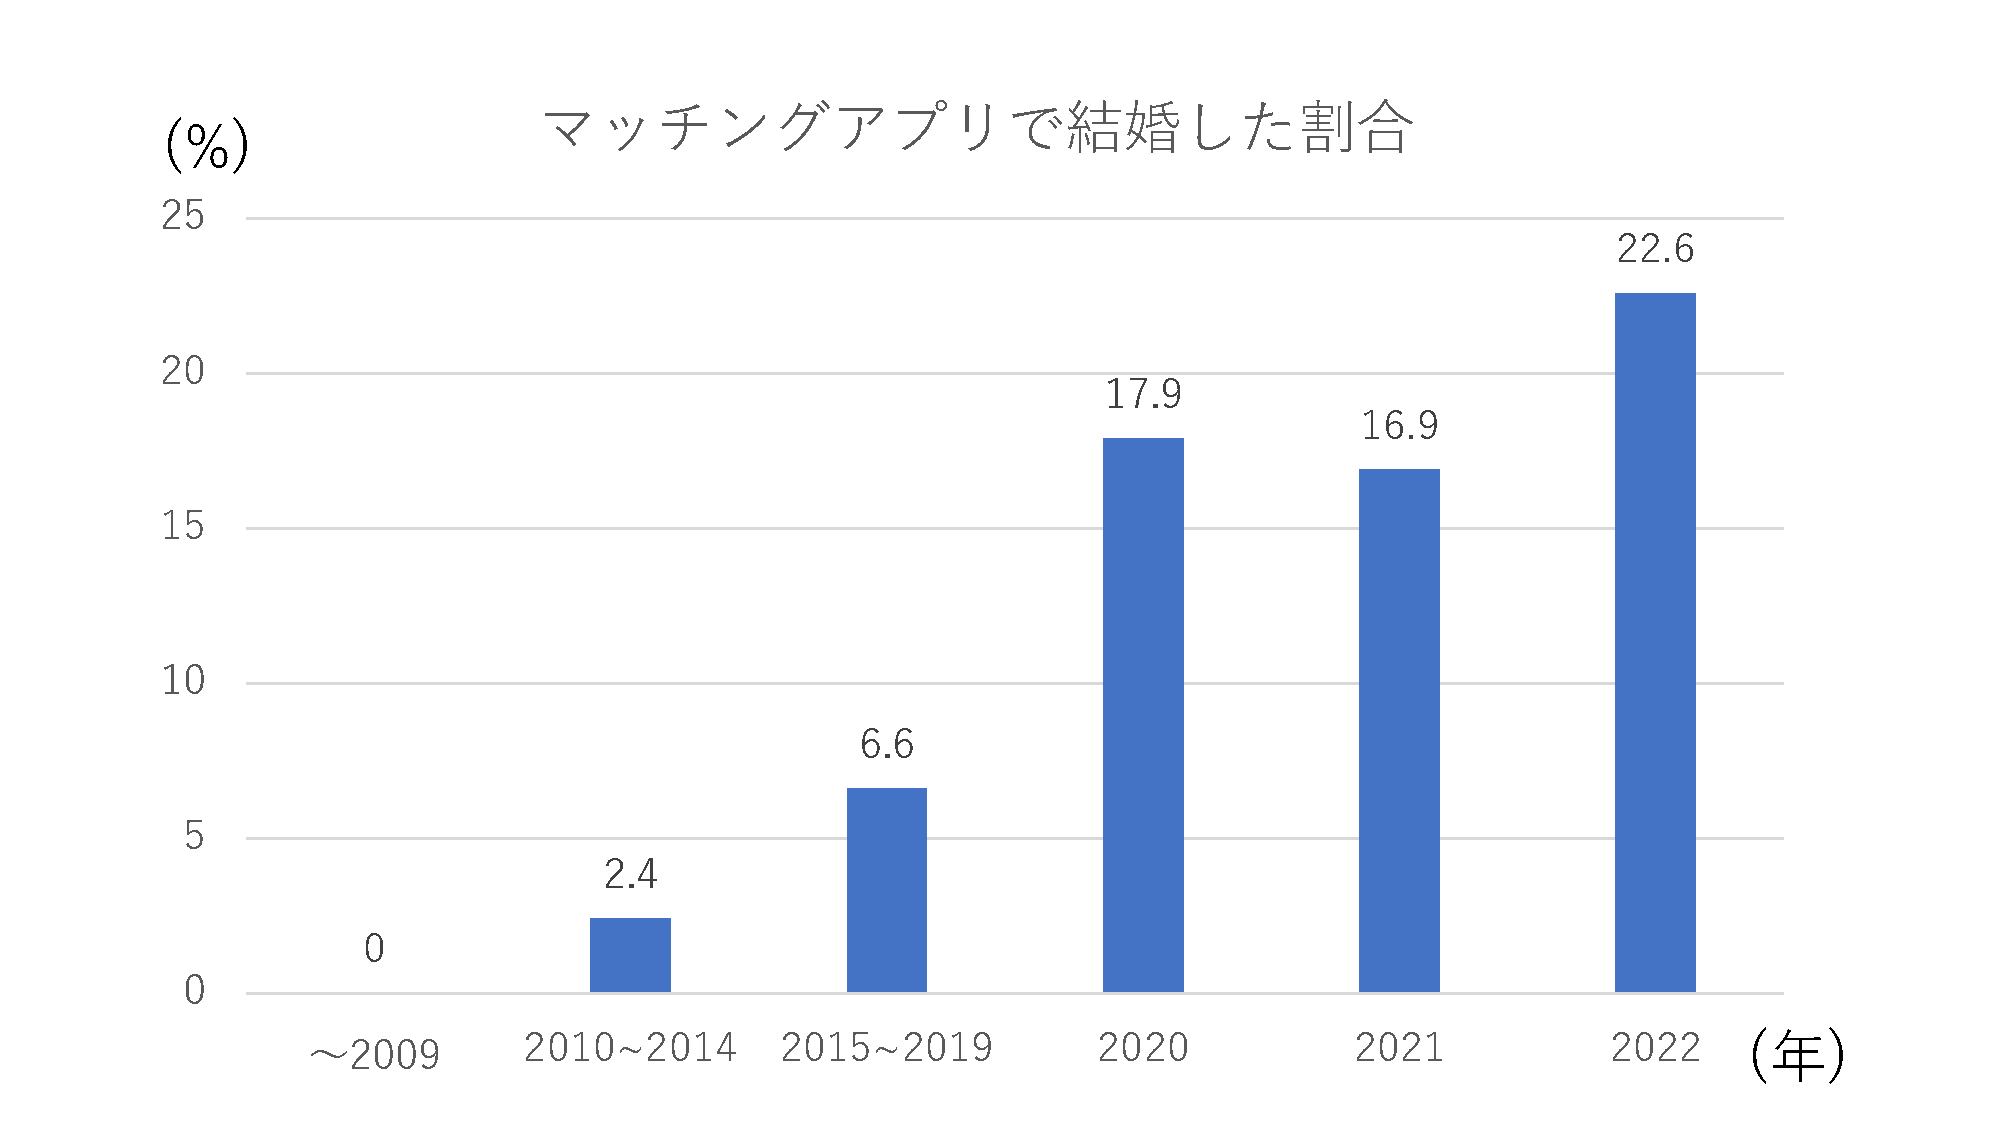
\includegraphics[keepaspectratio, scale=0.5]{mattinnguwariai.pdf}
\end{center}
 \caption{マッチングアプリで結婚した割合}
 \label{fig:mattingu}
\end{figure}
\clearpage

\section{アプリケーション提案}
少子化が引き起こす問題と少子化の実態,少子化は何が要因となっているかについてを説明させていただいた.
少子化の要因である出会いの減少の解決法としてマッチングアプリを利用してデートをするというものがある.しかしマッチングアプリで出会った相手とのデートは怖いなどの否定的なイメージを持たれており,そもそも経験が浅くデート自体が不安であると考える人もいる.

そこでVR空間を利用して1度仮想的なデートを実施し,直接会うまでをサポートできればデートに対する印象が変わるのではないかと考えた.
本研究では2人きりで会う恐怖を緩和し,デートに対する不安を軽減するために,仮想空間内でデートする環境を構築することを目的とする.

\clearpage
\section{基本技術について}
\subsection{VR}
VRはVirtual Realityの略で,人工現実感や仮想現実と訳されている.ここには「表面的には現実ではないが、本質的には現実」という意味が含まれ、VRによって「限りなく実体験に近い体験が得られる」ということを示している.

また,VRには,大きく分けると視聴型と参加型の2通りがある.
視聴型は流れている3D映像を見て、授業を受けたり医療の支援をしたりといった使い方が可能である.
一方,参加型のVRでは,映像の中を自由に歩き回るだけでなく,映像内のものを触ったり動かしたりすることもできる.そのため,観光事業や住宅販売において活用されている.
\subsection{HMD}
HMDはHead Mounted Display(ヘッドマウントディスプレイ)の略称であり,ゴーグルやヘルメット,メガネのように,頭部に装着するディスプレイ装置のことである.HMDには大きくわけて2種類の用途があり,ひとつは物理空間を必要とせず,超大画面の映像体験ができるディスプレイとしての用途である.もうひとつは視覚効果による3次元の演出である.

大画面ディスプレイ効果としては,左右のディスプレイがそれぞれ微妙な角度をつけて画像を表示しており,遠近法を利用することで目に錯覚を起こし小さなディスプレイを非常に大きいものとして認識するようになっている.このタイプのHMDは現在ほとんどの製品が販売を終了している.

3次元空間を演出するためのHMDは,左右のディスプレイに別の画像を表示してある.2つの画像は角度,色相が異なっており遠近法を利用することで,対象物が目前に立体物として存在するような錯覚を引き起こしている.
\subsubsection{Oculus Go}
Oculus Goは,Oculusが2018年5月に発売したスタンドアローン型のバーチャルリアリティ向けHMDである.従来のVRHMDと違い,PCやスマートフォンの接続を必要とせず,Oculus Go単体で扱う事ができる.

\subsection{Unity}
UnityとはUnity Technologiesが開発したゲーム開発プラットフォームであり,主にC\#を用いたプログラミングでコンテンツの開発が可能である。iOSやAndroid、XboxやPlayStation4などの様々なプラットフォームでの開発,VR/AR/MR機器向けのコンテンツ開発にも対応している。
\clearpage

\section{VRデートアプリについて}
\subsection{概要}
VR間で仮想的なデートを可能とするアプリケーションである.
マッチングアプリなどで文面上のコミュニケーションは取れたが異性と直接会うことに抵抗,恐怖を持つ方,まだデート経験が少なく,エスコートに慣れていない方がデートそのものに慣れるべく開発を行った.

\subsection{システム概要}\label{システム概要}
VR空間内でデートするアプリでは個別の問題点を以下のように改善するコンセプトを考案する.
まず,2人きりで会うことの不安については,VR空間内で擬似的にデートを行うことで改善できる.
アプリは時間が40分〜1時間程度に設定しており,自動進行としている.
自動進行の意図としては,デートの行動の制限し筋道を建てることでデート未経験者が失敗しないように配慮をしている.
デート時間の前半に共通の体験をしてもらい,後半はその体験についておしゃべりする時間としてお互いの性格を知る機会を設けることとした.

\subsection{VR内で会話機能のある類似アプリケーションについて} 
現在VRで実装され,本アプリケーションと最も類似するアプリケーションはVRChatである.

VRChatとは,VR空間内で多人数とのコミュニケーションを交わすことができる「ソーシャルVR」と呼ばれるジャンルのアプリケーションである.
VRChat内には内にはユーザが手がけた様々な「ワールド」と呼ばれるVR空間が用意されており、好きな場所で他のユーザとの交流を楽しむことができる。周囲にいるプレイヤーとはボイスチャットはもちろん、自分の身体の動きをアバターに反映させ、ボディーランゲージも可能となっている.
\subsection{VRデートアプリと類似アプリケーションについて}
VRChatは,VRChatは自由度が高く出来ることが多いためデート初心者にとっては何処に行けば良いのか,何をしたら良いのかの選択肢が広く計画を立てるのが困難である.

そこで,時間に制限をつけ,デートコースを制限することで既存のアプリにはないデートをしやすい環境をつくれるのではないかと考えた.

\subsection{開発に用いた技術}
本研究では以下の技術を用いて開発を行った.

・Unity2021.3.0f1
・C\#
・Oculus Go

\clearpage

\subsection{アプリ利用方法}
この節ではアプリの利用方法について記していく.
\subsubsection{URLの入力}
指定のURLをブラウザに入力すると図\ref{fig:kaisi}のような画面が映る.
\begin{figure}[h]
\begin{center}
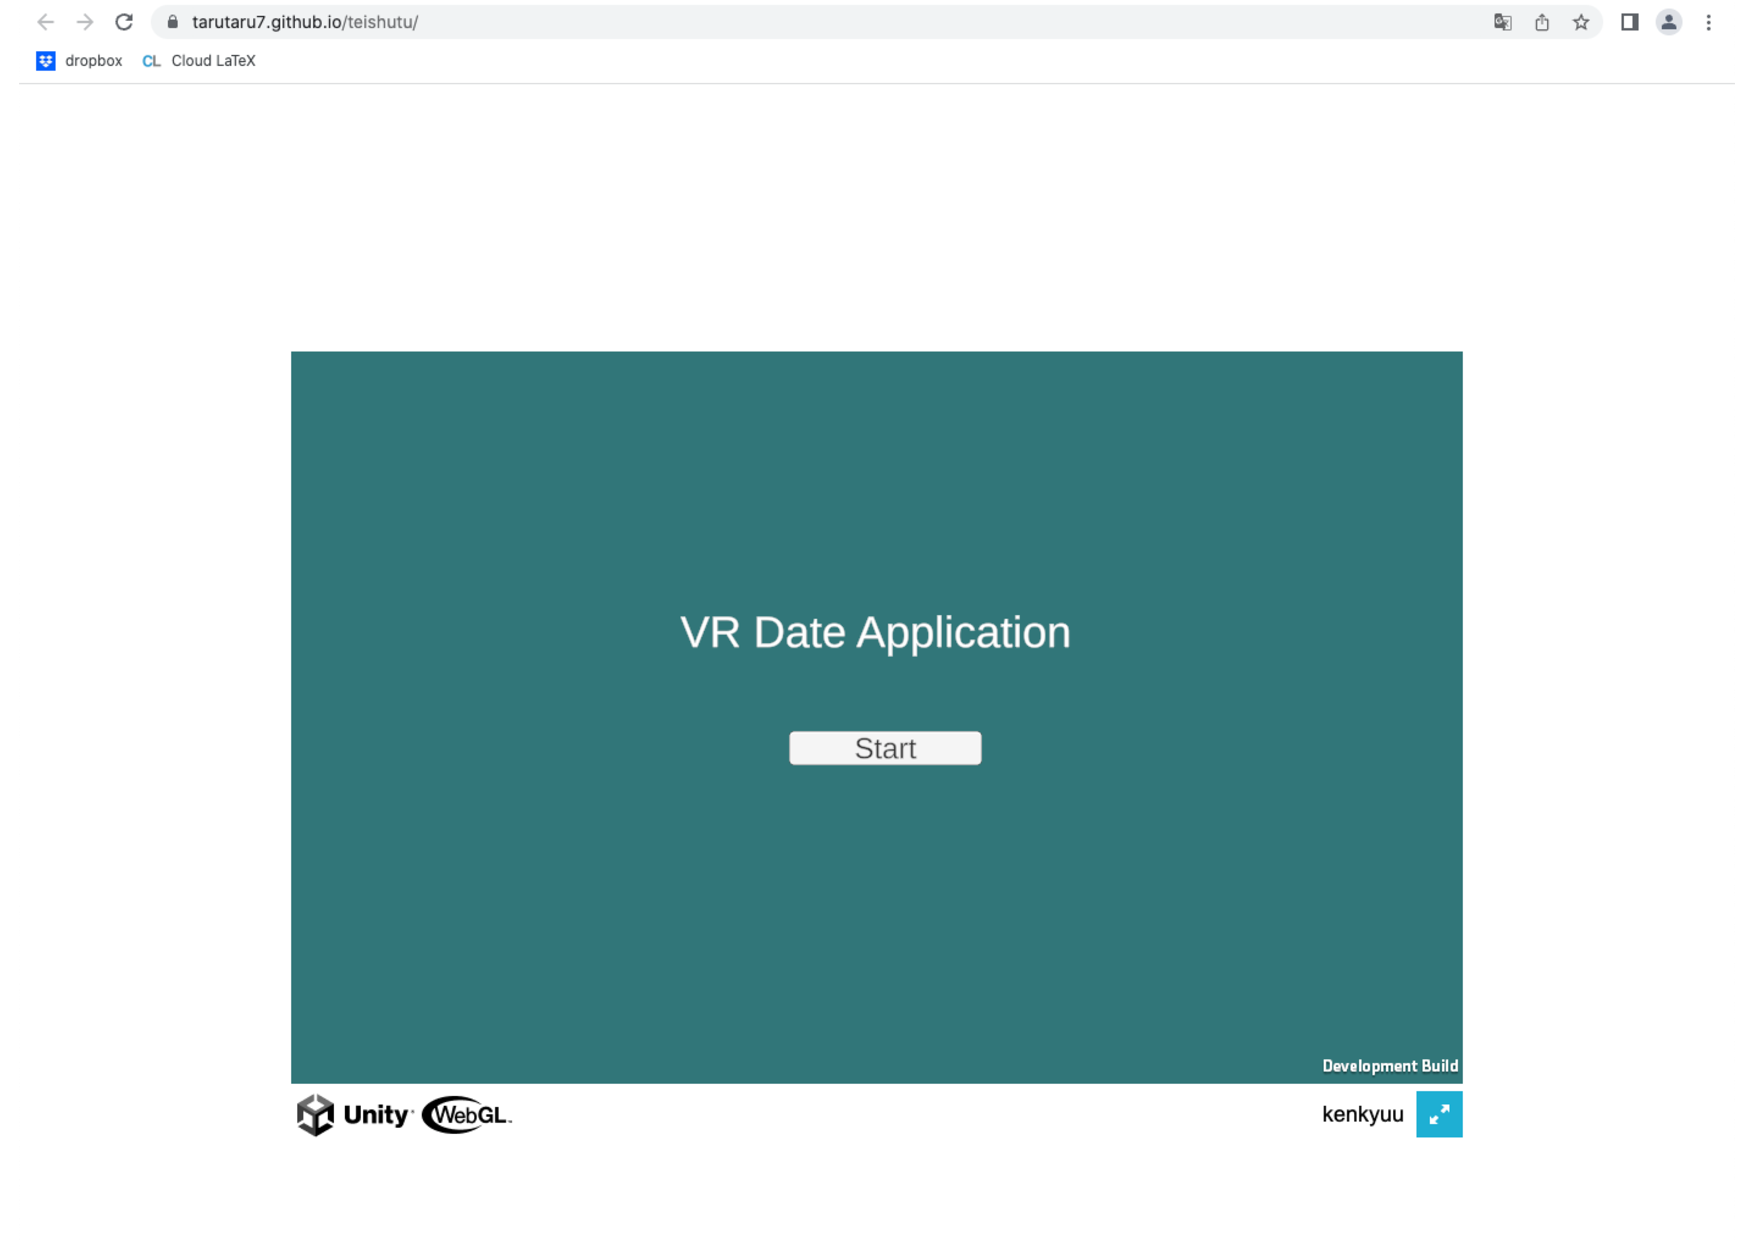
\includegraphics[keepaspectratio, scale=0.5]{apurikaisi.pdf}
\end{center}
 \caption{アプリ開始画面}
 \label{fig:kaisi}
\end{figure}

\clearpage

\subsubsection{アプリ開始画面}
図\ref{fig:kaisi}の中にあるstartボタンをクリックする事で図\ref{fig:yu-za-}に画面が切り替わる.
図\ref{fig:yu-za-}に切り替わった瞬間にデートがスタートする.
\subsubsection{アプリメイン画面}
図\ref{fig:yu-za-}のようにアプリが自動進行していき,その間ユーザ同士でアプリ内について話会う事ができる.

\begin{figure}[h]
\begin{center}
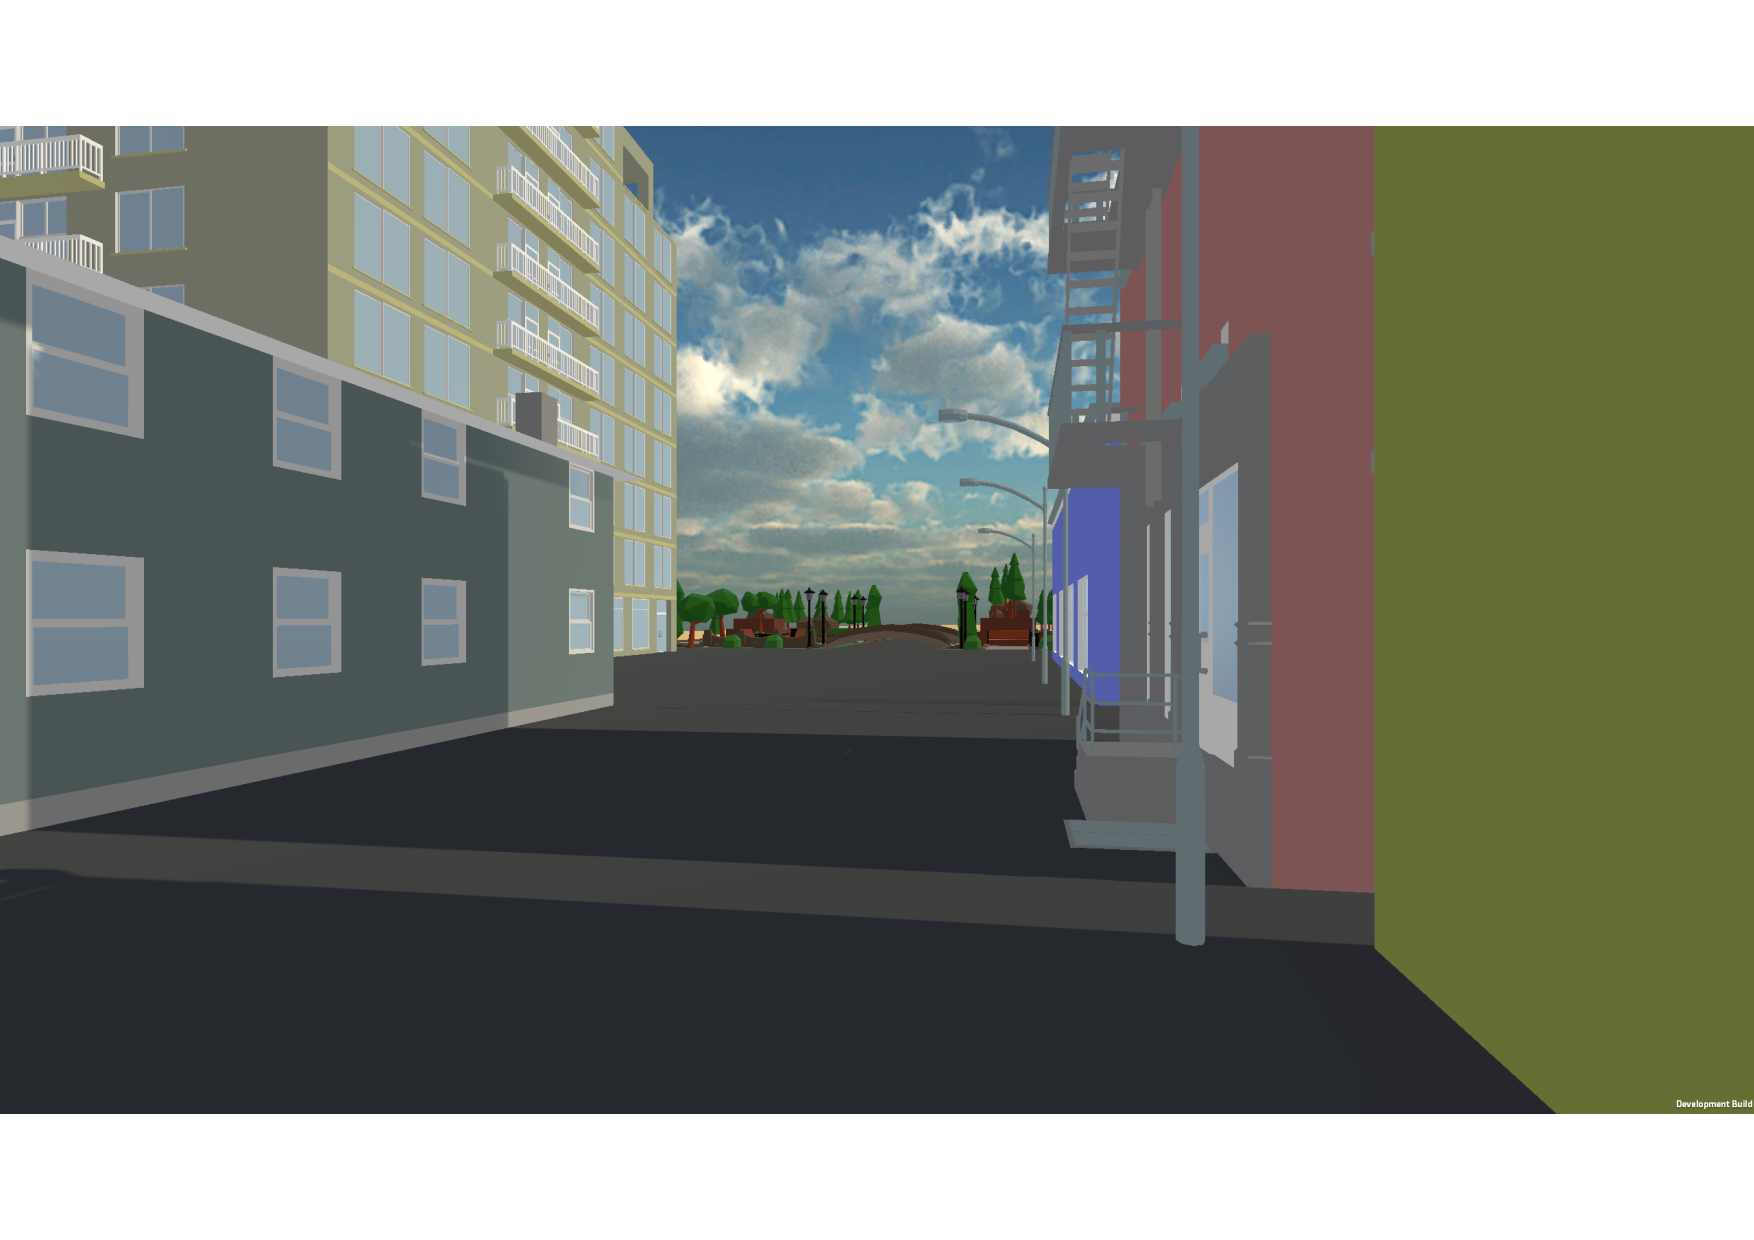
\includegraphics[keepaspectratio, scale=0.5]{yu-za-gamen.pdf}
\end{center}
 \caption{ユーザ視点の画面}
 \label{fig:yu-za-}
\end{figure}
\clearpage

\subsubsection{アプリ会話画面}
設定されたアプリの自動進行が終わると図\ref{fig:kissa}の画面に切り替わる.
この画面では,ユーザ同士が自動進行画面について思ったことを話すなどしてゆっくりと会話を楽染む事ができる

\begin{figure}[h]
\begin{center}
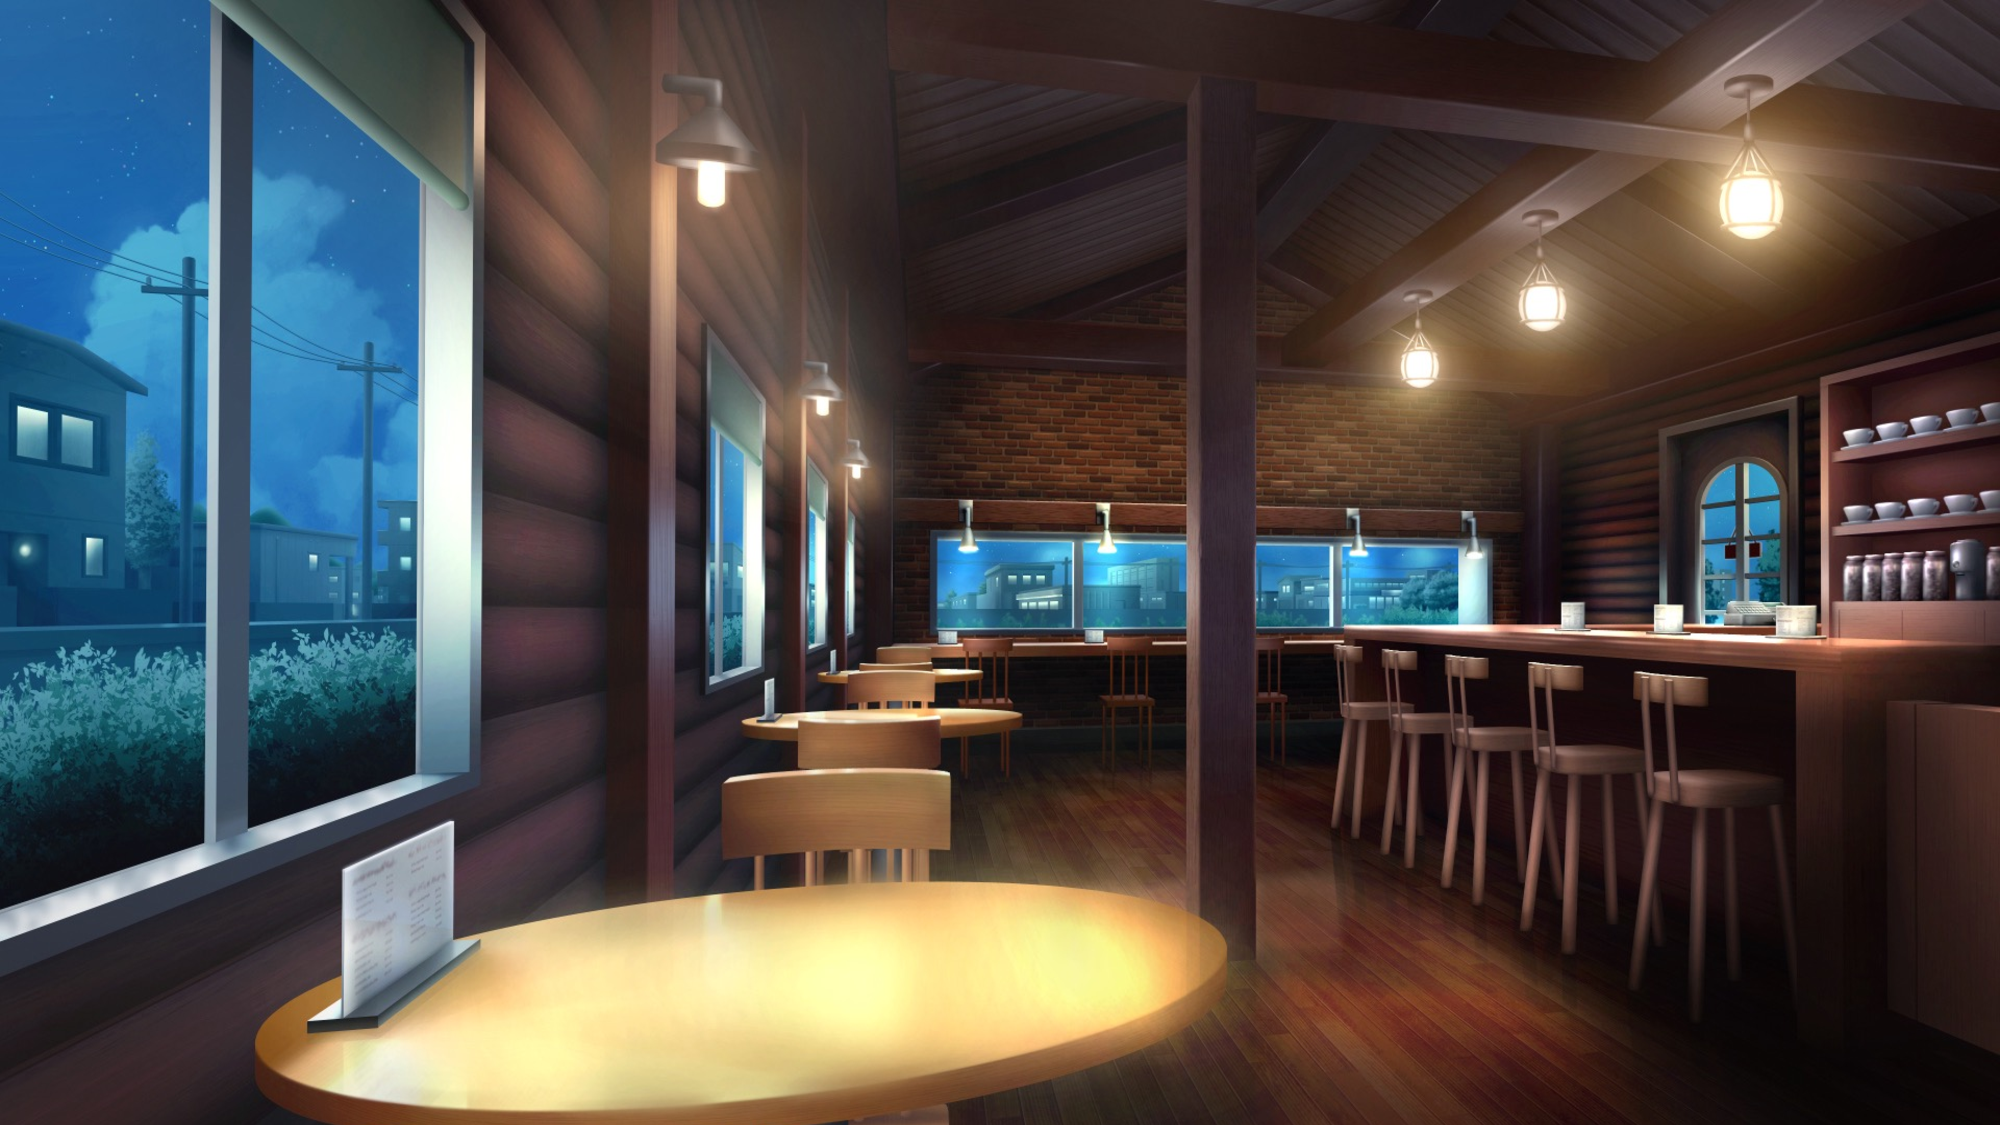
\includegraphics[keepaspectratio, scale=0.5]{kissatenn.pdf}
\end{center}
 \caption{アプリ会話画面}
 \label{fig:kissa}
\end{figure}


\clearpage


\section{システム実装}
\subsection{システム設計}
この節ではどのようにアプリケーションを作成したのかについて記していく.
\subsubsection{開発手順}
本研究では,アプリケーションの作成はゲーム開発エンジンであるUnityを用いた.

\label{sec:0}
\subsubsection{VR空間の設定}
本研究の目的としてデートの不安を軽減するとある.すなわち,デート自体に慣れるということであり,実際のデートを模す必要がある.そこで,VR空間内に動きが同期している男性アバターと女性アバターを作成し,デート環境が一般的なものであるものを用意した.

図\ref{fig:screen}は作成したVR空間を示し,①,②をそれぞれ男性アバター,女性アバターとした.
また,\ref{システム概要}にあるように③の方向に自動進行していく.

\begin{figure}[h]
\begin{center}
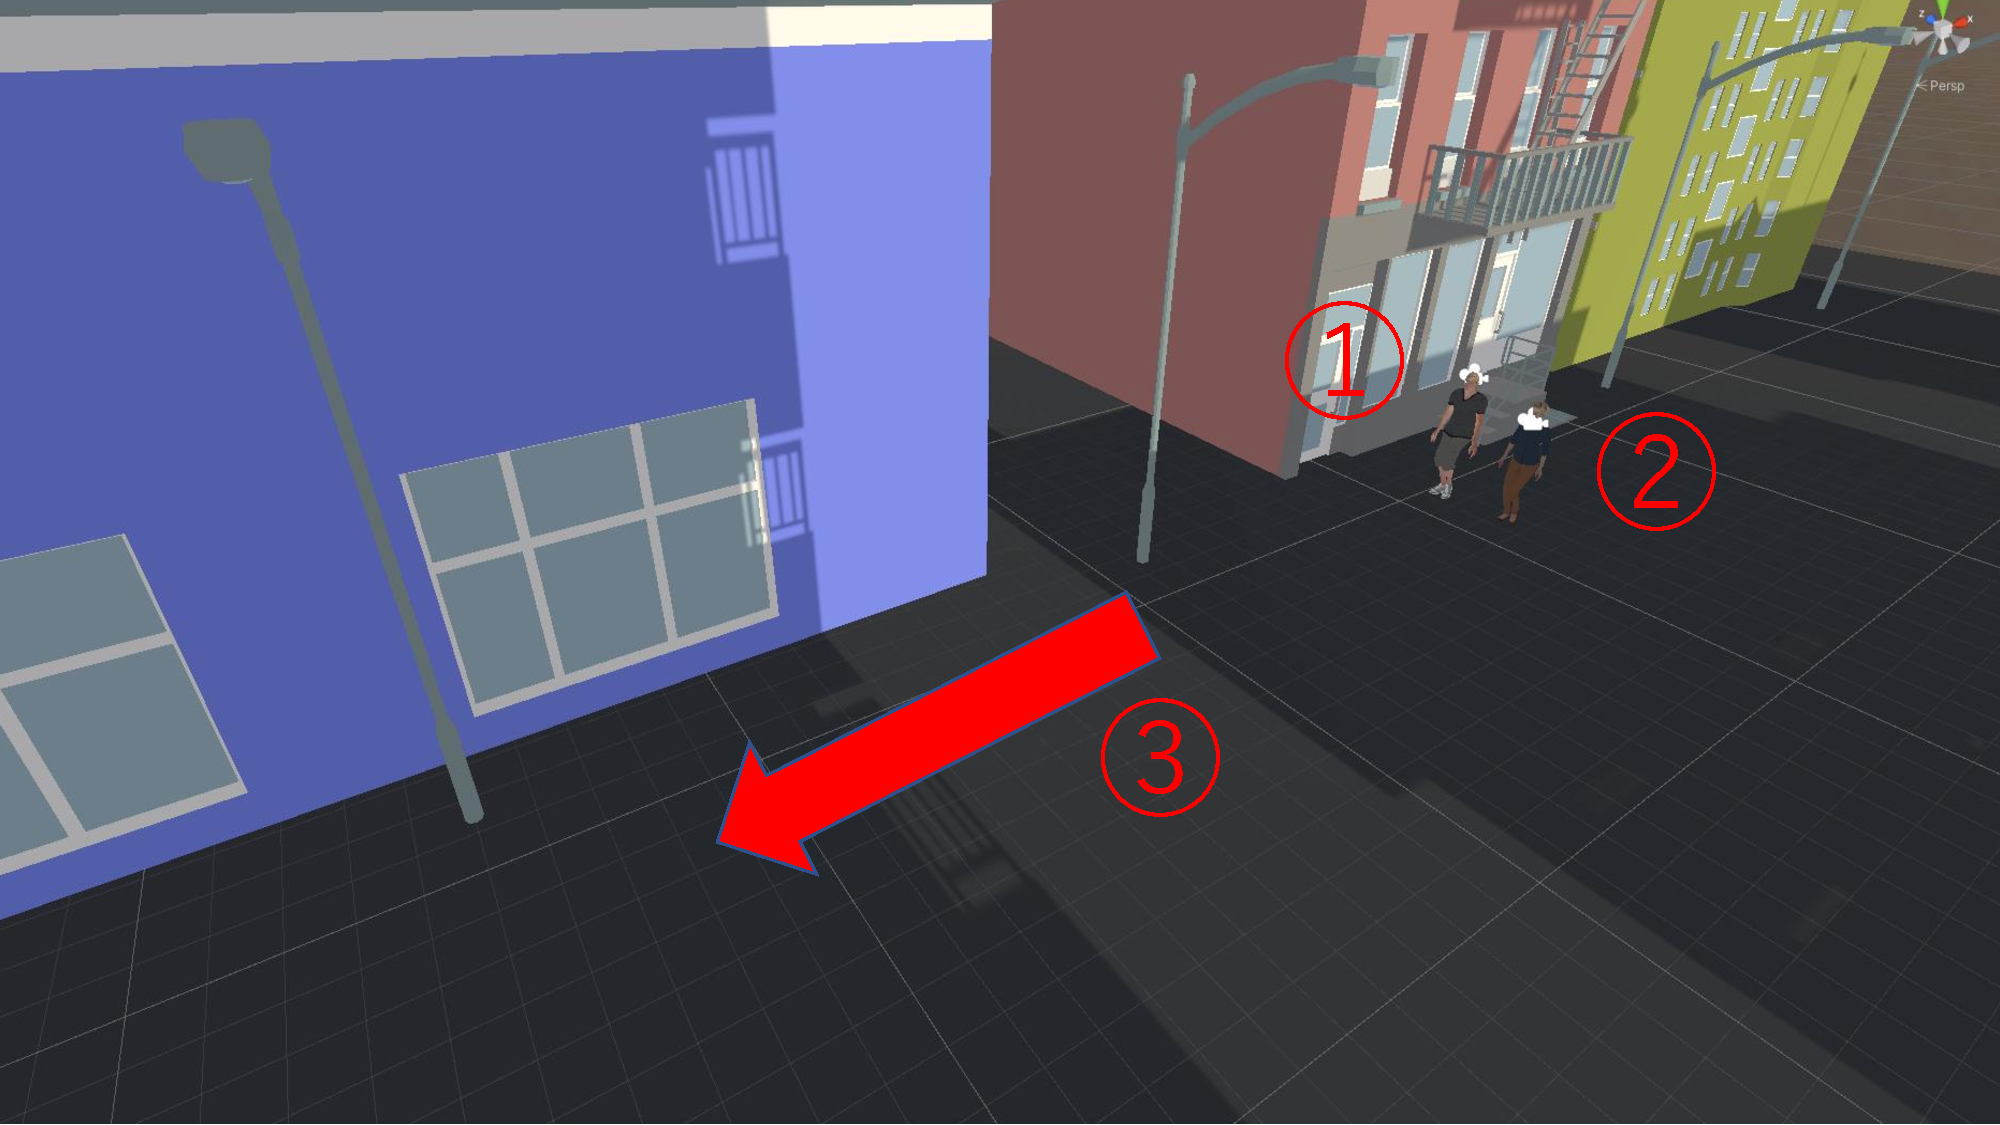
\includegraphics[keepaspectratio, scale=0.5]{screenshot.pdf}
\end{center}
 \caption{作成したVR空間}
 \label{fig:screen}
\end{figure}
\subsubsection{視点同期方法}
視点の同期はWebSocket-sharpを用いて実装した.
ユーザがブラウザに指定のURLを入力し,開始画面で待機する.
ユーザ同士の準備が完了したら同タイミングでアプリのスタートボタンを入力してもらい同期が完了となる.
\clearpage


\section{VRアプリに実装した技術}
この節ではアプリに実装した技術について記している.
\subsection{空の景色}
\subsubsection{Skybox}\label{SkyBox}
SkyBoxと呼ばれる空の景色を変えることができる機能を実装した.
この機能はDirectional Lightにアタッチすることで実装することができる.
また,SkyBoxのスクリプトに5種類の空の景色を入れて時間帯で入れ替わるようにすることで早朝,朝,昼,夕方,夜と現実に近い空間をつくることに成功した.
ソースコード\ref{shadow}はSkyBoxのスクリプトを示している.
\subsubsection{影}
\ref{SkyBox}で記したように空の景色を変更させたが,より現実に近い環境を作るため影も実装した.
実装方法はソースコード\ref{Sky}にあるようにDirectional Lightの角度を時間で変更するに設定することで可能とした.
\subsubsection{空のソースコード}

空のソースコードをソースコード\ref{Sky}に示す.
\begin{lstlisting}[caption=Sky,label=Sky]
using System.Collections;
using System.Collections.Generic;
using UnityEngine;

public class SkySystem : MonoBehaviour {

    [SerializeField]
    private float sunPos;
    
    public Material[] skybox;
    
    void Update()
    {
        
        transform.eulerAngles = new Vector3(sunPos, 0, 0);

        sunPos += Time.deltaTime * 20;
       
        if (sunPos >= 0 && 72 > sunPos)
            RenderSettings.skybox = skybox[0];
      
        else if (sunPos >= 72 && 144 > sunPos)
            RenderSettings.skybox = skybox[1];

        else if (sunPos >= 144 && 216 > sunPos)
            RenderSettings.skybox = skybox[2];

        else if (sunPos >= 216 && 288 > sunPos)
            RenderSettings.skybox = skybox[3];

        else if (sunPos >= 288 && 360 > sunPos)
            RenderSettings.skybox = skybox[4];
      
        if (sunPos > 360)
            sunPos = 0;
    }
}
\end{lstlisting}

\subsection{自動進行}
UnityのGameObjectに複数のPointを作成し,Pointをアバターが追従することで自動進行システムを作成できた.

\subsection{左右の視点移動操作}
ユーザが視線を共有するために左右の視点移動操作を実装した.
VR空間内であればHMDを傾ければ視線を変えられるが,PCからアプリケーションに接続した時のことを考え左右の矢印キーの入力で視線を変えられるようにした.
実装方法はソースコード\ref{siten}にあるようにRigidbodyをアタッチしたモデルに対してtrasform.Rotateで押した際にどの程度傾くのかを設定をして実装した.
\subsubsection{視点移動のソースコード}
\begin{lstlisting}[caption=視点移動,label=siten]
using System.Collections;
using System.Collections.Generic;
using UnityEngine;
using System;
using UnityEngine.SceneManagement;


public class ManController : MonoBehaviour
{
    // Start is called before the first frame update
   
    private Rigidbody manRigidbody;
  

    void Start()
    {
        manRigidbody = GetComponent<Rigidbody>();
    }

    // Update is called once per frame
    void Update()
    {
        
        if (Input.GetKey("right"))
        {
            manRigidbody.transform.Rotate(0, 3, 0);
        }
        else if (Input.GetKey("left"))
        {
            manRigidbody.transform.Rotate(0, -3, 0);
        }
    
    }

}
\end{lstlisting}

\clearpage

\section{開発環境}
\subsection{使用言語}
\subsubsection{C\#}
制御構文などに高水準言語の特徴を持ちながら、ハードウェア寄りの記述も可能な低水準言語の特徴も併せ持つ。基幹系システムや、動作環境の資源制約が厳しい、あるいは実行速度性能が要求されるソフトウェアの開発に用いられることが多い。後発のC++やJava、C\#など、「C系」と呼ばれる派生言語の始祖でもある.

\subsection{通信プロトコル}
\subsubsection{WebSocket}
WebSocketとは、ブラウザとウェブサーバーとの間で双方向通信を行うための通信プロトコルである.
サーバー側とユーザー側が常にオンライン状態を維持することによって、双方向通信を可能としている.
そのため,従来の通信プロトコルと比べ,リアルタイムに情報共有することを可能としている\cite{wecsocketsetumi}.
\clearpage

\section{結言}
2015年9月に開催された「国連持続可能な開発サミット」でSDGsが掲げられた.この中に少子化も含まれており,その要因は,晩婚化の進展\cite{sasaki2012},交際率・婚姻率の減少\cite{naikakufu2019}などとされている.

実際に日本では,20年間で平均初婚年齢は2.6歳(男性)/3.1歳(女性)増加している.
しかし,結婚意欲は僅かに減少している程度でほぼ変化していない.
すなわち,「結婚はしたいけれど,良い相手に恵まれない」との考えが大多数を占めている\cite{naikakufu2019}.

過去には学校や職場,友人を通じた出会いが有ったが,最近では出会いの場としてSNSを活用する者やマッチングアプリの利用者が増加している.
しかし,知らない人と2人きりで会うことに恐怖を感じたり,初デートに不安を感じるデート未経験者も少なくない\cite{prtimes,yoshimura2020}.

本研究では,異性と直接会うことに抵抗,恐怖を持つ方,まだデート経験が少なく,エスコートに慣れていない方がデートそのものに慣れるためのアプリケーションを開発した.このアプリケーションを使用することで2人きりで会う恐怖を緩和し,デートに対する不安を軽減することが期待される.また,今後このアプリケーションを使用してもらい,どの程度恐怖や不安が軽減されたのか評価してもらいたい.

\clearpage



\section{謝辞}
本研究の遂行及び本論文の作成にあたり,須田研究室の仲間に多くの手助けを頂きました,深く感謝の意を表します.そして,本論文の作成にあたり多大なる御指導及び御助言を頂きました,須田宇宙准教授に深く感謝の意を表します.

\clearpage

%参考文献
\begin{thebibliography}{99}
\bibitem{sasaki2012} 佐々木 尚之: ``不確実な時代の結婚-JGSSライフコース調査による潜在的稼得力の影響の検証'', 「家族社会学研究」,第24号,pp152-164(2012)
\bibitem{naikakufu2019} 内閣府: ``少子化対策の現状'', \url{https://www8.cao.go.jp/shoushi/shoushika/whitepaper/measures/w-2016/28webhonpen/html/b1_s1-1-3.html}, 2023/1/16参照
\bibitem{doukou}国立社会保障・人口問題研究所:``第15回出生動向基本調査'',
\url{https://www.ipss.go.jp/ps-doukou/j/doukou15/NFS15_report3.pdf},2023/1/14参照
\bibitem{prtimes}PRTIMES:``マッチングアプリは怖い?危ない目に合った?初めて会うまでの期間は!?徹底調査'',
\url{https://prtimes.jp/main/html/rd/p/000000016.000059676.html},2023/1/14参照
\bibitem{huuhuutyousa}「いい夫婦の日」に関するアンケート調査:``明治安田生命 NEWS RELEASE'',
\url{https://www.meijiyasuda.co.jp/profile/news/release/2022/pdf/20221116_01.pdf},2023/1/16参照
\bibitem{wecsocketsetumi}WebSocketとは?WebSocketについて詳しく解説します:``Web会議の基礎知識'',
\url{https://www.freshvoice.net/knowledge/word/6323/},2023/1/10参照
\end{thebibliography}

\end{document}
